\documentclass[11pt, aspectratio=169]{beamer}
% \documentclass[11pt,handout]{beamer}
\usepackage[T1]{fontenc}
\usepackage[utf8]{inputenc}
\usepackage{textcomp}
\usepackage{float, afterpage, rotating, graphicx}
\usepackage{epstopdf}
\usepackage{longtable, booktabs, tabularx}
\usepackage{fancyvrb, moreverb, relsize}
\usepackage{eurosym, calc}
\usepackage{amsmath, amssymb, amsfonts, amsthm, bm}
\usepackage[
    natbib=true,
    bibencoding=inputenc,
    bibstyle=authoryear-ibid,
    citestyle=authoryear-comp,
    maxcitenames=3,
    maxbibnames=10,
    useprefix=false,
    sortcites=true,
    backend=bibtex
]{biblatex}
\AtBeginDocument{\toggletrue{blx@useprefix}}
\AtBeginBibliography{\togglefalse{blx@useprefix}}
\setlength{\bibitemsep}{1.5ex}
\addbibresource{refs.bib}

\hypersetup{colorlinks=true, linkcolor=black, anchorcolor=black, citecolor=black, filecolor=black, menucolor=black, runcolor=black, urlcolor=black}

\setbeamertemplate{footline}[frame number]
\setbeamertemplate{navigation symbols}{}
\setbeamertemplate{frametitle}{\centering\vspace{1ex}\insertframetitle\par}


\begin{document}

\title{Topics in Behavioural Decision  Theory}

\author[Christian Hilpert]
{
{\bf Christian Hilpert}\\
{\small Lingnan College, Sun Yat-sen University}\\[1ex]
}


\begin{frame}
    \titlepage
    \note{~}
\end{frame}

\frame{\frametitle{Agenda}
\tableofcontents
}

\frame{\frametitle{Agenda}
\tableofcontents[currentsection]
}

%        \item Application and Limits of CPT\bigskip
   %     \item Alternative Theories\bigskip

\begin{frame}{Literature}
    \begin{itemize}
        \item \citet{Barberis2017Talk} AEA lecture\bigskip
        \item \citet{Thaler2016}\bigskip
        \item \citet{Barberis2013a}\bigskip
        \item \citet{Wakker2010}, Cambridge University Press, ''Prospect Theory for Risk and Ambiguity''\bigskip
	\end{itemize}
\end{frame}

\section{Brief Overview of Behavioural Economics}
\begin{frame}{Brief overview}
    1950s-1990s: ''Traditional Finance''\bigskip
\begin{itemize}
	\item psychological shortcomings \bigskip
    \item new way of thinking about finance questions\bigskip
        \begin{enumerate}
            \item insurance\medskip
            \item portfolio choice\medskip
            \item corporate finance\ldots
            \medskip
        \end{enumerate}
    \item not alternative to mainstream economics (Micro)\bigskip
\end{itemize}
\end{frame}

\begin{frame}{Some questions}
    \begin{itemize}
        \item Why do people buy insurance, gamble, and hold stocks?\bigskip
        \item Why do people hold on to losing stocks?\bigskip
        \item Why are IPOs underpriced?\bigskip
    \end{itemize}
\end{frame}

\begin{frame}{Standard paradigm}
    \begin{itemize}
        \item $t= 0,1,2,...$ time\bigskip
        \item $S_t$ possible states\bigskip
        \item $p(s_t)$ probability of $s_t \in S_t$ occurring in $t$\bigskip
        \item $X_t$ payoff/consumption in $t$\bigskip
    \end{itemize}
\end{frame}

\begin{frame}{Standard paradigm}
\begin{itemize}
    \item Agent-utility function $U(X\mid S)$\medskip
    \begin{itemize}
\item time-independent discount factor $\delta $\medskip
\item implicitly: von-Neumann/Morgenstern axioms\medskip
\end{itemize}\bigskip

    \item Maximise expected lifetime utility\medskip
	\[\max_{x_t} \sum_t  \delta^t \left(\sum_{s_t \in S_t} U(x_t \mid s_t)\rho (s_t) \right) \qquad \text{s.t.} \quad x_t \in X_t\]
   \end{itemize}
\end{frame}


\begin{frame}{Behavioural decisions}
\begin{itemize}
\item Adjust optimisation:
	\[\max_{x_t} \sum_t  \delta^t \left(\sum_{s_t \in S_t} U(x_t \mid s_t)\rho (s_t) \right) \qquad \text{s.t.} \quad x_t \in X_t\]\bigskip
        \item Non-standard preferences: $U$, $\delta $\bigskip
        \item Non-standard beliefs: $\rho$\bigskip
        \item Non-standard decision making: $\max$\bigskip
\end{itemize}
\end{frame}


\begin{frame}{Alternative theories of choice under risk}
    \begin{enumerate}
        \item Reference-dependence, prospect theory, ambiguity\medskip
        \begin{itemize}
        \item Implies: loss aversion, non-standard time preferences, self-control issues, time inconsistency, social preferences
        \end{itemize}\bigskip
        \item Overconfidence, extrapolation, experience effects\medskip
         \begin{itemize}
        \item Implies: overestimation, confirmation bias, projection bias, law of small numbers.  \end{itemize}\bigskip
        \item Bounded rationality, cognitive limitations.\medskip
        \begin{itemize}
        \item Implies: rules of thumb, simplification, framing
        \end{itemize}\bigskip
    \end{enumerate}

    Not sharply separated.  1 weakest, 3 strongest departure  from EU
\end{frame}

\begin{frame}{Alternatives}
    \begin{itemize}
        \item Bounded rationality\bigskip
        \item Evolutionary game theory\bigskip
        \item Decision theory (unawareness, unforeseen contingencies)\bigskip
    \end{itemize}\bigskip
\end{frame}
\begin{frame}{Behavioural economics is controversial!}
    \begin{itemize}
        \item poor experimental standards\medskip
        \item departure from revealed preference approaches\medskip
        \item anything goes\medskip
    \end{itemize}
\end{frame}

\section{Cumulative Prospect Theory}
\frame{\frametitle{Agenda}
\tableofcontents[currentsection]
}
\begin{frame}{Prospect Theory and Cumulative Prospect Theory}
    \begin{itemize}
        \item Most finance models assume expected utility theory to evaluate risks\bigskip
        \item Experimentally, at least, not a good fit\bigskip
        \item \citet{KahnemanTversky1979}: prospect theory\bigskip
        \item \citet{TverskyKahneman1992}: cumulative prospect theory\bigskip
        \item Alternatives: disappointment aversion, rank-dependent utility, salience theory, regret theory, SP\&A theory\bigskip
    \end{itemize}
\end{frame}


\begin{frame}{Prospect Theory and Cumulative Prospect Theory}
    \begin{itemize}
        \item A reference-dependent utility function is a family $\{U(\cdot \mid \gamma):x \longrightarrow \mathbb{R} \mid \gamma \in X\}$  of utility functions over $X$ indexed by $\gamma \in X$.\bigskip
        \item The utility $U(X \mid \gamma)$ describes the utility of the consumption and the reference point is $\gamma$.\bigskip
        \item Prospect theory vs expected utility theory: Consider gamble $L = (X, p, y, q)$\bigskip
        \item  $EU=p V(w +x)+qV(w+y)$\bigskip
       \item $PT=w(p)V(x)+w(q)V(y)$\bigskip
\end{itemize}
\end{frame}


\begin{frame}{Expected utility}
\centering
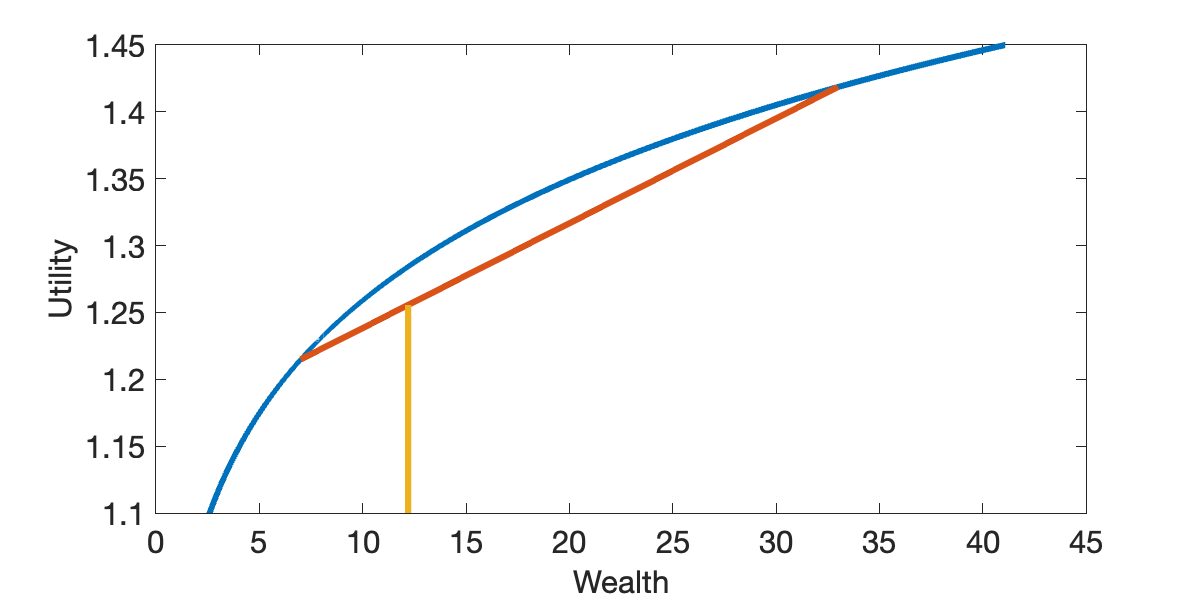
\includegraphics[width= 0.99\textwidth]{expected_utility}
\end{frame}

\begin{frame}{Cumulative prospect theory value function}
\centering
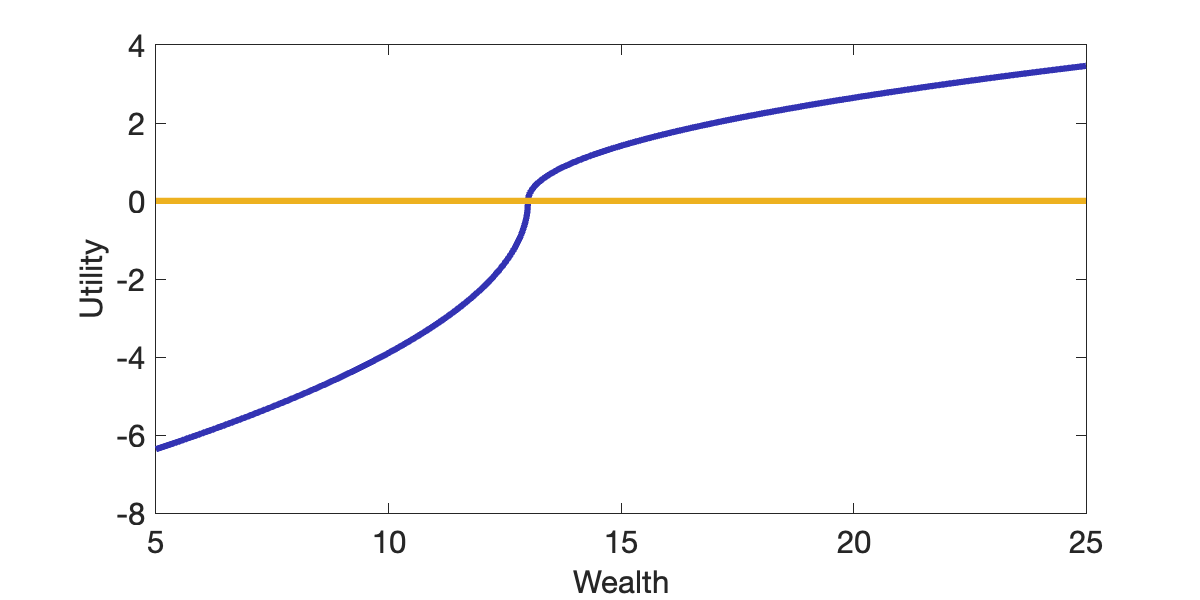
\includegraphics[width= 0.99\textwidth]{cpt_utility}
\end{frame}


\begin{frame}{Four key features}
    \begin{enumerate}[1.]
        \item Reference-dependence:\bigskip
            \begin{itemize}
                \item Gains and losses instead of final wealth\medskip
                \item Experimental evidence consistent with perception of alternative\medskip
            \end{itemize}\bigskip
        \item Loss aversion:\bigskip
            \begin{itemize}
                \item $V(x)$ has a kink in zero.\medskip
                \item Losses loom larger than gains.\medskip
                \item Evidence: $(110,\frac{1}{2},-100,\frac{1}{2})$ is unattractive.
            \end{itemize}
    \end{enumerate}
\end{frame}

\begin{frame}{Four key features}
    \begin{enumerate}[3.]
        \item Diminishing sensitivity\bigskip
            \begin{itemize}
                \item $V(\cdot)$ is concave over gains, convex over losses\medskip
                \item Evidence: $(500,1) \succ (1000,\frac{1}{2})$ and
                \qquad  $(-500,1) \preceq  (-1000,\frac{1}{2})$
            \end{itemize}
            \bigskip
    \end{enumerate}
    \begin{enumerate}[4.]
        \item Probability weighting:\bigskip
            \begin{itemize}
                \item Transform probability with decision weights $w(\cdot)$:
                high weight on low probabilities\medskip
                \item Evidence: $(5,1)\prec (5000,0.001)$ lottery\\
                \qquad  $(-5,1)\succ (-5000,0.001)$ insurance\medskip
            \item Note: $w$ are decision weights not beliefs
        \end{itemize}

    \end{enumerate}
\end{frame}




\begin{frame}{Cumulative Prospect Theory (Tversky and Kahneman, 1992)}
    \begin{itemize}
        \item \citet{TverskyKahneman1992} address some limitations (FOSD) of the original \citet{KahnemanTversky1979} prospect theory \bigskip
        \item They apply probability weighing to the cumulative distribution function\bigskip
        \item Example: gain at least 50, lose 100 or more\bigskip
        \item Formally, consider
        \[(x_{-m},p_{-m},...,x_{-1},p_{-1},x_0,p_0,x_1,p_1,...,x_n,p_n)\]
        with $x_i < x_j$ for $i<j,x_0=0$\bigskip
         \end{itemize}
\end{frame}

\begin{frame}{Cumulative Prospect Theory (Tversky and Kahneman, 1992)}
    \begin{itemize}
       \item The value assigned equals
        \[ \sum_{i=-m}^{n} \pi_i V(x_i)\]
        with\\
            \begin{equation}
                \pi_i = \begin{cases}
                w(p_i+...+p_n) - w(p_i+...+p_n),  & 0\leq i \leq  n\\
                w(p_{-m}+...+p_i) - w(p_{-m}+...+p_{i-1}),  & -m\leq i \leq 0\\
            \end{cases}
            \end{equation}\bigskip
        \item Individuals overweight fails of a probability distribution\bigskip
        \item Preserves a taste for lottery like gambles\bigskip
    \end{itemize}
\end{frame}

\begin{frame}{Cumulative prospect theory decision weights}
\centering
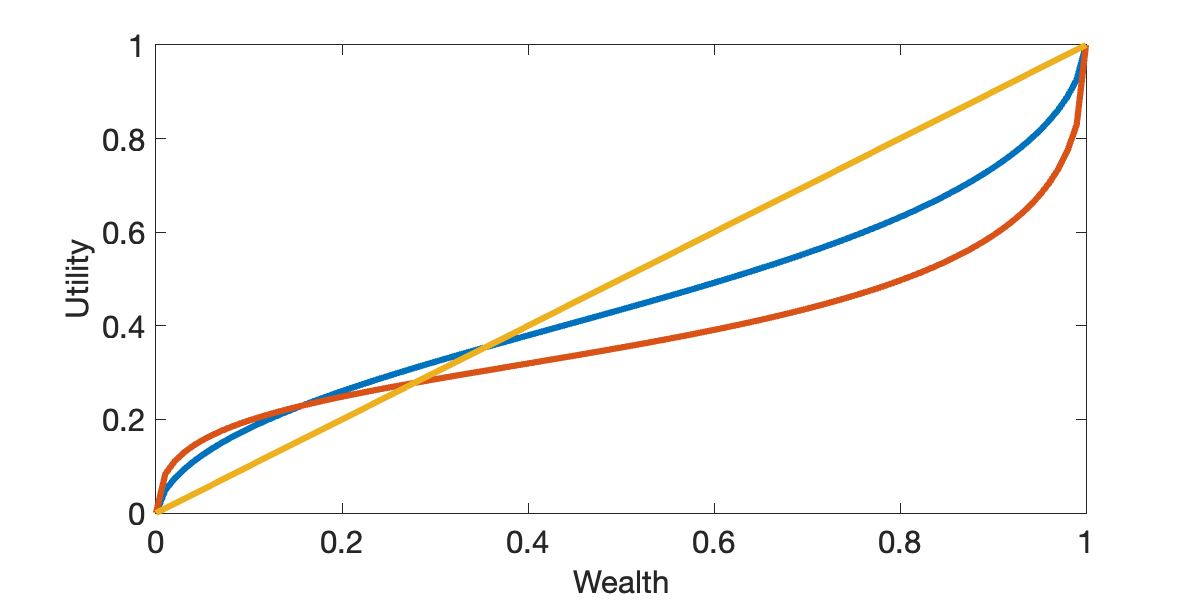
\includegraphics[width= 0.99\textwidth]{cpt_weights}
\end{frame}

\begin{frame}{Cumulative Prospect Theory (Tversky and Kahneman, 1992)}
    \begin{itemize}
        \item \citet{TverskyKahneman1992} suggest:
\begin{equation}
    V(x) = \begin{cases}
    x^\alpha,  & x\geq 0\\
    -\lambda (-x)^\alpha,  & x< 0\\
    \end{cases}
\end{equation}\medskip
\item with \[w(p) = \frac{p^{\delta}}{(p^{\delta}+(1-p)^{\delta})^{\frac{1}{\delta}}}\]
\item Their (questionable) estimates are $\alpha =0.88$, $\lambda =2.25$, and  $\delta =0.69$\medskip
    \item There are alternatives to formalize $w$.
\end{itemize}
\end{frame}


\begin{frame}{Challenges and discussion - value function}
    \begin{itemize}
        \item How to define gains and losses?\bigskip
        \item Total wealth, financial wealth, stock holdings, individual stocks?\bigskip
        \item what is a gain:\medskip
        \begin{itemize}
            \item exceeds zero?\medskip
            \item risk-free rate?\medskip
            \item expectation?\medskip
        \end{itemize}
                \item Diminishing sensitivity  $\Rightarrow$ \citet{Rabin2000}'s critique (not as important feature theoretically)\medskip
        \end{itemize}
        \end{frame}

      \begin{frame}{Challenges and discussion - decision weights}
    \begin{itemize}
        \item Probability weighting in many applications more important than loss aversion\medskip
        \item Overweighting vs underweighting: black swan events: Taleb (2007)\medskip
        \item There is evidence for both cases\medskip
        \item Could be either \medskip
        \begin{itemize}
        \item Decision from description $\Rightarrow$ overweighting\smallskip
        \item Decision from experience $\Rightarrow$ underweighting\smallskip
        \end{itemize}
        \item not clear how to interpret:\medskip
          \begin{itemize}
        \item overestimation (belief) $\Rightarrow$ mistake\smallskip
        \item overweighting (preference) $\Rightarrow$ not mistake???\smallskip
        (some evidence fro preference)
           \end{itemize}
    \end{itemize}
\end{frame}


\begin{frame}[allowframebreaks]
    \frametitle{References}
    \renewcommand{\bibfont}{\normalfont\footnotesize}
    \printbibliography
\end{frame}

\end{document}
